\documentclass[../main.tex]{subfiles}

\begin{document}

Descargue de Sicuaplus el archivo de Excel con el nombre \textit{DatosRegresion.xls}. Allí encontrará información relacionada con la contaminación atmosférica en 38 ciudades de Estados Unidos. Las variables que se presentan en el archivo son las siguientes:

\begin{itemize}
  \item Contenido de $SO_2$ (Dióxido de Azufre) en el aire. Esta variable se mide en microorganismos por metro cúbico.
  \item Número de fábricas con más de 20 empleados.
  \item Número de habitantes (miles).
  \item Velocidad media del viento al año (millas por hora).
  \item Precipitación media anual (litros por pulgada).
  \item Número medio de días con lluvia al año.
\end{itemize}

Estime el modelo de regresión lineal múltiple para la variable Contenido de $SO_2$ en el aire usando todas las variables descritas. Para esto de respuesta a los siguientes literales:

\begin{enumerate}[(a)]

\item \textbf{(2 puntos)} Escriba a continuación el modelo de regresión lineal que le permite predecir el Contenido de $SO_2$ en el aire con base en las variables independientes.

\begin{center}
  \begin{tabular}{ | l | c | }
    \hline
    $Y$ & Contenido de$ SO_2$ en el aire (microorganismos por metro cúbico) \\ \hline
    $X_1$ & Número de fábricas con más de 20 empleados \\ \hline
    $X_2$ & Numéro de habitantes (miles) \\ \hline
    $X_3$ & Velocidad media del viento al año (millas por hora) \\ \hline
    $X_4$ & Precipitación media anual (Litros por pulgada) \\ \hline
    $X_5$ & Número medio de días con lluvia al año \\
    \hline
  \end{tabular}
\end{center}

El modelo es:
$$Y = \beta_0 + X_1 \beta_1+ X_2 \beta_2+ X_3 \beta_3+ X_4 \beta_4+ X_5 \beta_5$$

\pagebreak

\item \textbf{(10 puntos)} Realice una gráfica de dispersión entre cada una de las variables
independientes y la dependiente. Indique, para cada caso, si de manera visual se puede
percibir una relación lineal.

\begin{figure}[h]
\centering
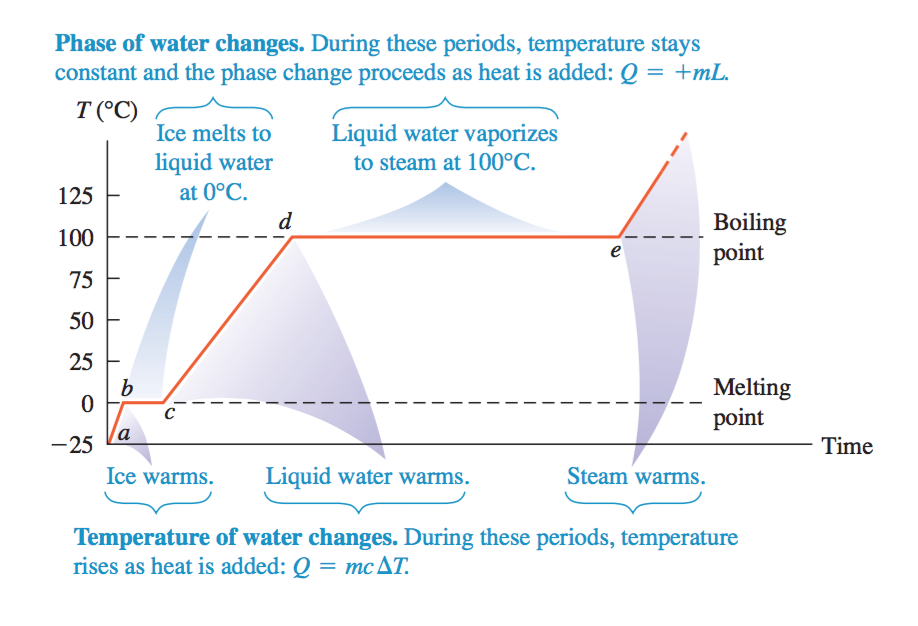
\includegraphics[width=13cm]{plot.png}
\label{fig:img1}
\end{figure}

En la gráfica se muestra la relación entre cada una de las variables predictoras y la variable independiente, en $x2$, $x3$, $x4$ y $x5$ se observa una estrecha relación lineal, mientras que en $x1$ no tanto.

\pagebreak

\item \textbf{(4 puntos)} Con ayuda de SPSS, presente a continuación la tabla de ANOVA, y la tabla de coeficientes.

A continuación, se muestra la tabla ANOVA, con los valores por cada una de las variables predictoras (los valores de regresión son la suma de estos, los totales, la suma de estos anteriores y los residuales). Las tablas fueron realizadas usando el lenguaje de programación R.

\begin{table}[ht]
\centering
\begin{tabular}{lrrrrr}
  \hline
 & Df & Sum Sq & Mean Sq & F value & Pr($>$F) \\ 
  \hline
x1 & 1 & 9403.34 & 9403.34 & 38.57 & 0.0000 \\ 
  x2 & 1 & 3630.47 & 3630.47 & 14.89 & 0.0005 \\ 
  x3 & 1 & 41.72 & 41.72 & 0.17 & 0.6819 \\ 
  x4 & 1 & 109.57 & 109.57 & 0.45 & 0.5074 \\ 
  x5 & 1 & 845.94 & 845.94 & 3.47 & 0.0717 \\ 
  Residuals & 32 & 7802.22 & 243.82 &  &  \\ 
   \hline
\end{tabular}
\end{table}

\begin{table}[ht]
\centering
\begin{tabular}{rrrrr}
  \hline
 & Estimate & Std. Error & t value & Pr($>$$|$t$|$) \\ 
  \hline
(Intercept) & 19.0293 & 20.6876 & 0.92 & 0.3645 \\ 
  $x1$ & 0.0721 & 0.0162 & 4.45 & 0.0001 \\ 
  $x2$ & -0.0469 & 0.0155 & -3.02 & 0.0049 \\ 
  $x3$ & -1.7276 & 2.0105 & -0.86 & 0.3966 \\ 
  $x4$ & -0.1336 & 0.2581 & -0.52 & 0.6083 \\ 
  $x5$ & 0.2481 & 0.1332 & 1.86 & 0.0717 \\ 
   \hline
\end{tabular}
\end{table}

La tabla ANOVA es:

\bigskip
\begin{tabular}{ |p{2cm}||p{2.5cm}|p{1cm}|p{2cm}|p{1.8cm}|  }
 \hline
 \multicolumn{5}{|c|}{ANOVA} \\
 \hline
 Model & Sum of squares & gl & Mean Square & F\\
 \hline
 Regression   & 14031.01    &5&   14031.01 & $57.55$\\
 Residual   & 7802.22    &32&   $243.82$ &\\
 Total   &   21833.23  &37&   $301.37$ &\\
 \hline
\end{tabular}

\item \textbf{(4 puntos)} Para aquellos coeficientes que resultan significativos, presente la interpretación correspondiente a cada uno.

Los coeficientes significativos son según la prueba anterior y la tabla ANOVA, $x_1$ y $x_2$. Lo cuál significa que el nñumero de fabricas con más de 20 empleados y el número de habitantes, cuyos coeficientes de significancia $\beta_1$ y $\beta_2$ son respectivamente 0.0721 y -0.04669 contribuyen positiva y negativamente respectivamente sobre la predicción del contenido de $SO_2$ en el aire.

\item \textbf{(2 puntos)} Estime el valor del coeficiente de determinación, e interprételo.

El coeficiente de determinación $R^2$, es 0.6426. Es decir, el modelo es significativo para predecir, es decir, el modelo explica $y$ usando las variables usadas y posee gran capacodad explicativa y predictiva.


\item \textbf{(8 puntos)} Verifique los supuestos del modelo de regresión lineal múltiple. Para ello, utilizando SPSS, realice una prueba de bondad de ajuste sobre los errores estimados del
modelo de regresión lineal múltiple.

\begin{figure}[h]
\begin{tabular}{cc}
  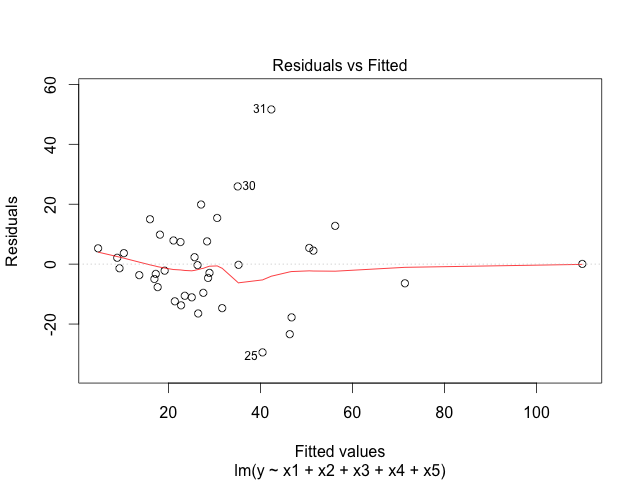
\includegraphics[width=6cm]{fit1} &   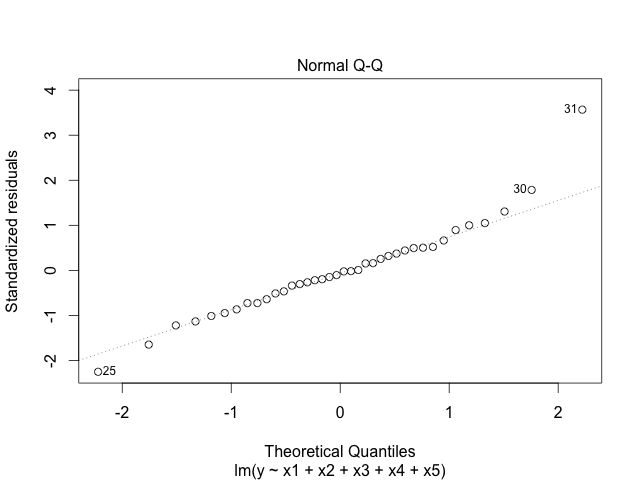
\includegraphics[width=6cm]{fit2} \\
(a)  & (b) Ajuste de cuantiles del error \\[6pt]
 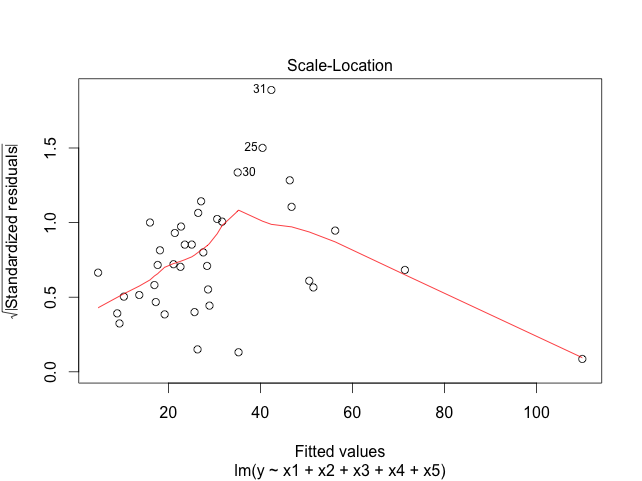
\includegraphics[width=6cm]{fit3} &   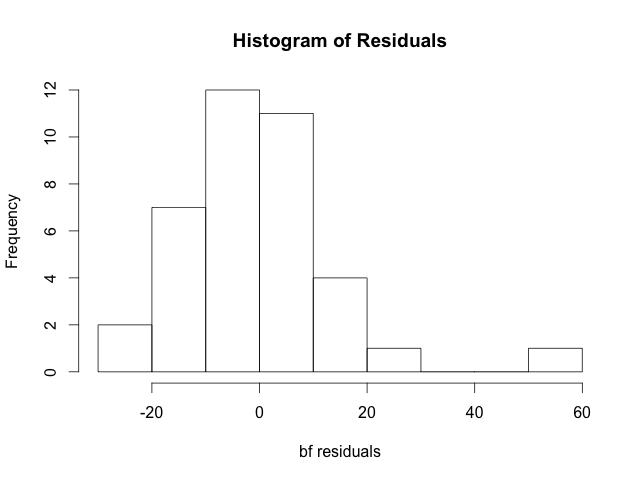
\includegraphics[width=6cm]{fit4} \\
(c)  & (d) Histograma de los errores
\end{tabular}
\caption{}
\end{figure}

Por medio de la gráfica anterior, se concluye que el error distribuye normal con media cero y varianza constante.

\end{enumerate}
\end{document}
